\documentclass[conf]{new-aiaa}
%\documentclass[journal]{new-aiaa} for journal papers
\usepackage[utf8]{inputenc}

\usepackage{graphicx}
\usepackage{amsmath}
\usepackage[version=4]{mhchem}
\usepackage{siunitx}
\usepackage{longtable,tabularx}
\usepackage{float}
\usepackage{listings}
\usepackage{color} %red, green, blue, yellow, cyan, magenta, black, white
\definecolor{mygreen}{RGB}{28,172,0} % color values Red, Green, Blue
\definecolor{mylilas}{RGB}{170,55,241}
\setlength\LTleft{0pt} 

% ================================================================ % 
\title{ASE 389P.4 Methods of Orbit Determination \\ Homework 0: Numerical Integration Tool}

\author{Junette Hsin}
\affil{Masters Student, Aerospace Engineering and Engineering Mechanics, University of Texas, Austin, TX 78712}

\begin{document}

\maketitle

\begin{abstract}
This assignment is designed to provide a basic introduction on how to use a numeric integrator. MATLAB was used to complete the assignment. 
\end{abstract}

% ================================================================ % 
\section{Problem 1}

\subsection{Statement} 
\begin{center}
\fbox{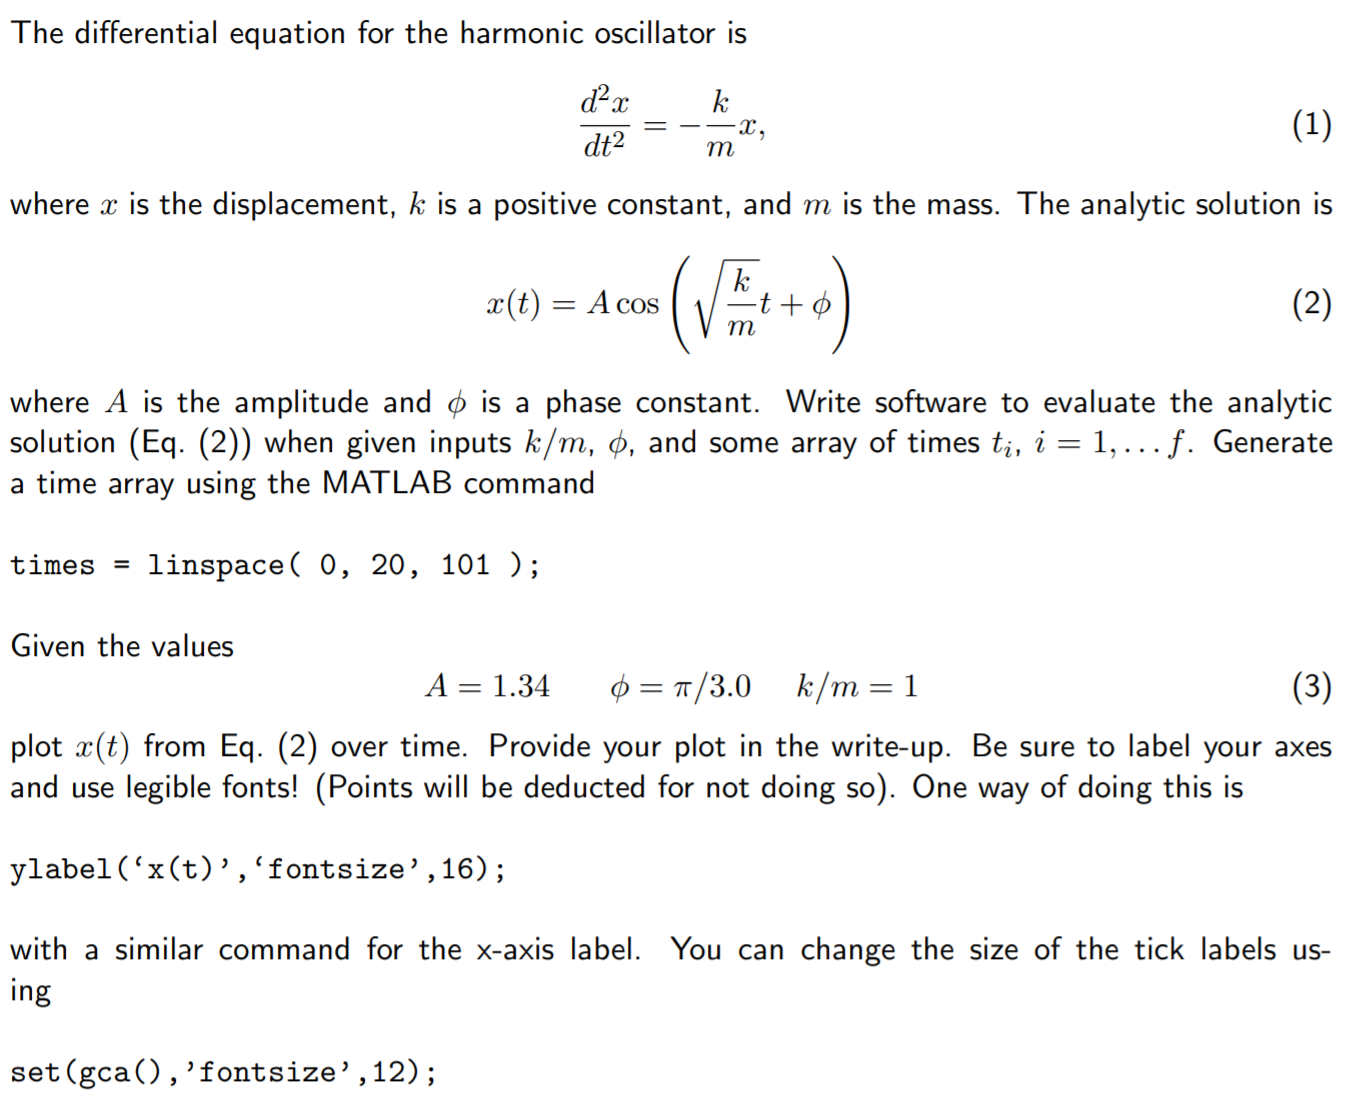
\includegraphics[width=0.9\textwidth]{prob_1.png}} \\
\end{center}

% -------------------------------- % 
\newpage
\subsection{Solution} 

For a harmonic oscillator with the analytic solution 

\begin{equation}
	x(t) = A ~cos \Bigg( \sqrt{ \frac{k}{m} } t + \phi \Bigg)
\end{equation}

Given the values 

\begin{equation}
	A = 1.34 ~~~~~~~~\phi = \pi/3.0 ~~~~~~~~k/m = 1
\end{equation}

The plot for $x(t)$ over a time interval of 20 seconds is shown in Figure \ref{fig:xt}: 

\begin{figure}[H]
	\centering
	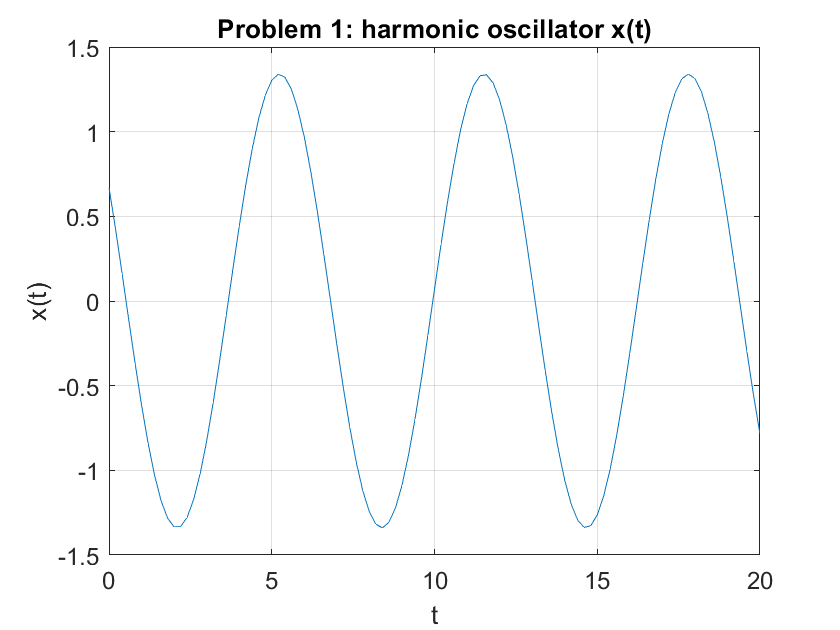
\includegraphics[width=0.7\textwidth]{prob1_xt.png}
	\caption{}
	\label{fig:xt}
\end{figure}



% ================================================================ % 
\section{Problem 2} 

\subsection{Statement} 
\begin{center}
\fbox{
\includegraphics[width=0.9\textwidth]{prob_2.png}} \\
\end{center}

% -------------------------------- % 
\subsection{Solution} 

An analytical solution provides an exact solution but may not always be easily computed or even possible to obtain, such as in the case of some complex differential equations. Numerical solutions provide approximations which may not exactly match the analytical solution, but can come close within allowable tolerances while being more computationally efficient to obtain. 

The accuracy of the MATLAB ordinary differential equations solver \texttt{ode45} can be adjusted by modifying the options structure through the function \texttt{odeset} \cite{ode45}. RelTol, the relative accuracy tolerance, controls the number of correct digits in the computed answer, and AbsTol, the absolute error tolerance, controls the difference between the computed answer and the true solution \cite{odeset}. Figure \ref{fig:reltol12} shows the error between the numerical and analytical solutions to the displacement of the harmonic oscillator for a relative tolerance of 1e-12, which matches the order of magnitude of the error. When the relative tolerance is adjusted to 1e-6 in Figure \ref{fig:reltol6}, the order of magnitude of the error adjusts accordingly. 

\begin{figure}[H]
	\centering
	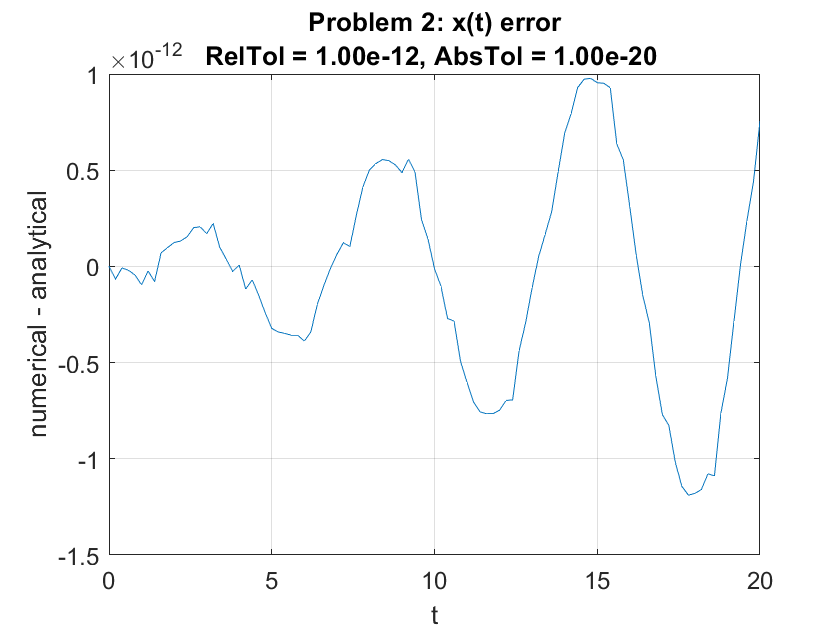
\includegraphics[width=0.7\textwidth]{prob2_err_reltol12.png}
	\caption{}
	\label{fig:reltol12}
\end{figure}

The error grows over time because MATLAB ODE solvers are set up as initial value problems in which the solution at each step is obtained iteratively by propagating the state of the previous step, beginning at the initial conditions \cite{choose_ode}. The truncation of digits and error from numerical integration is propagated as well at each step. 

\begin{figure}[H]
	\centering
	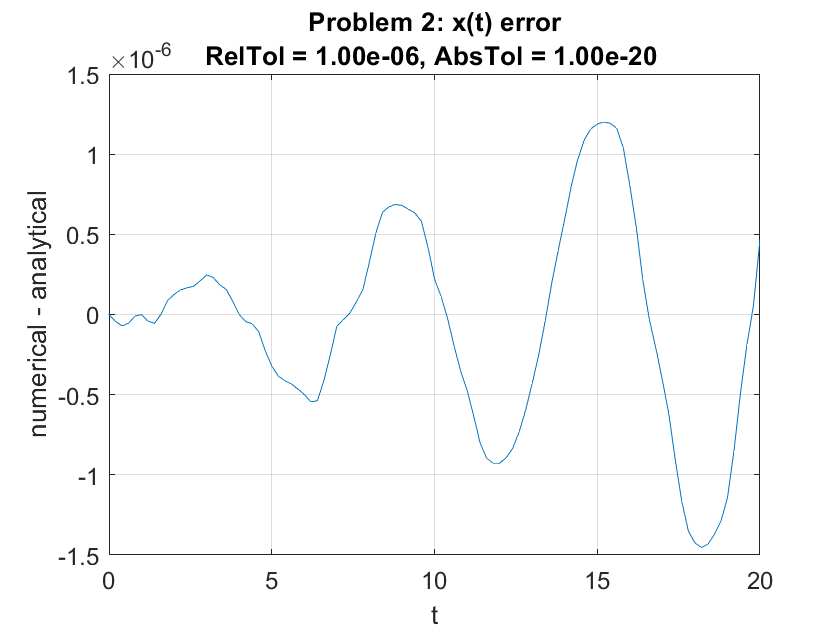
\includegraphics[width=0.7\textwidth]{prob2_err_reltol6.png}
	\caption{}
	\label{fig:reltol6}
\end{figure}


% ================================================================ % 

\newpage
\section{Appendix} 

HW0 MATLAB code: 



\lstset{language=Matlab,%
	%basicstyle=\color{red},
	breaklines=true,%
	morekeywords={matlab2tikz},
	keywordstyle=\color{blue},%
	morekeywords=[2]{1}, keywordstyle=[2]{\color{black}},
	identifierstyle=\color{black},%
	stringstyle=\color{mylilas},
	commentstyle=\color{mygreen},%
	showstringspaces=false,%without this there will be a symbol in the places where there is a space
	numbers=left,%
	numberstyle={\tiny \color{black}},% size of the numbers
	numbersep=9pt, % this defines how far the numbers are from the text
	emph=[1]{for,end,break},emphstyle=[1]\color{red}, %some words to emphasise
	%emph=[2]{word1,word2}, emphstyle=[2]{style},    
}

\begin{lstlisting}[basicstyle=\footnotesize]
% ASE 389 Orbit Determination
% HW 0
% Junette Hsin 


%% Problem 1 

t   = linspace( 0, 20, 101 ); 
t   = 0 : 0.2 : 400; 
A   = 1.34; 
phi = pi/3; 
km  = 1; 

x   = A * cos( sqrt( km )*t + phi ); 

name = 'Problem 1: harmonic oscillator x(t)'; 
figure('name', name); 
plot(t, x); 
ylabel('x(t)'); 
xlabel('t'); 
title(name); 
set(gca, 'fontsize', 12); 


%% Problem 2 

y0 = zeros(2,1); 
y0(1) = A * cos(phi); 
y0(2) = - A * sqrt( km ) * sin(phi); 

reltol = 1e-12; 
abstol = 1e-20; 
myoptions   = odeset( 'RelTol', reltol, 'AbsTol', abstol); 
[t, y]      = ode45( @harmoscillator, t, y0, myoptions, km); 

% numerical - analytical 
error = y(:,1)' - x; 

name = 'Problem 2: x(t) error'; 
figure('name', name); 
plot(t, error); 
xlabel('t')
ylabel('numerical - analytical')
title({name ;
sprintf('RelTol = %.2e, AbsTol = %.2e ', reltol, abstol) }); 
set(gca, 'fontsize', 12); 


%% subfunctions 

function dx = harmoscillator( t, x, km )

dx    = zeros(2, 1); 
dx(1) = x(2); 
dx(2) = -km * x(1); 

end 
\end{lstlisting}


% ================================================================ % 
\newpage
\bibliography{sample}

\end{document}
